	In this chapter, we review bipartite graphs and matchings and then discuss their relevance to 
	this thesis. We will also begin our discussion of linear programming, in a casual way, 
	to give the reader a taste for what is to come in subsequent chapters.
\begin{section}{Bipartite Graphs and Matchings}

	Throughout this thesis, we will be interested in a specific subclass of graphs known as 
	bipartite graphs. Unless otherwise noted, our algorithms will assume a bipartite structure.

	\begin{definition}
		A \emph{bipartite graph} is a graph whose vertices can be partitioned into two 
		sets $U$ and $V$ such that all edges connect a vertex $u\in U$ to a vertex $v\in V$.
		We will denote this graph $G = (U,V,E)$, where $E$ is a subset of $(U\times V)$.
	\end{definition}	
	\begin{figure}[h]
		\centering
	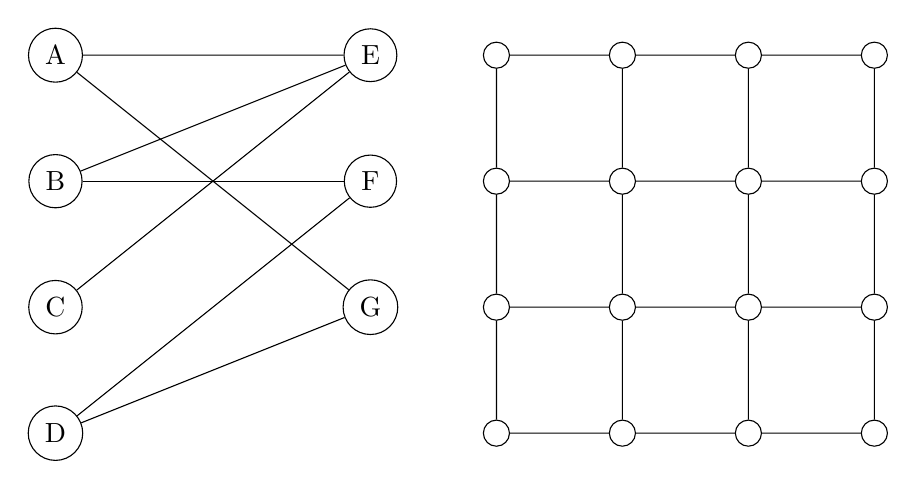
\begin{tikzpicture}[scale=.8,auto=left,every node/.style={circle,draw=black}]
		%left nodes
		\node (n1) at (1,10) {A};
		\node (n2) at (1,8) {B};
		\node (n3) at (1,6) {C};
		\node (n4) at (1,4) {D};

		%right nodes
		\node (n5) at (6,10) {E};
		\node (n6) at (6, 8) {F};
		\node (n7) at (6, 6) {G};
		
		%edges
		\draw (n1) -- (n5);
		\draw (n1) -- (n7);
		\draw (n2) -- (n5);
		\draw (n2) -- (n6);
		\draw (n3) -- (n5);
		\draw (n4) -- (n6);
		\draw (n4) -- (n7);

		%left nodes
		\node (n1) at (8,10) {};
		\node (n2) at (8,8) {};
		\node (n3) at (8,6) {};
		\node (n4) at (8,4) {};

		%center left nodes
		\node (n5) at (10,10) {};
		\node (n6) at (10,8) {};
		\node (n7) at (10,6) {};
		\node (n8) at (10,4) {};

		%center right nodes
		\node (n9) at (12,10) {};
		\node (n10) at (12,8) {};
		\node (n11) at (12,6) {};
		\node (n12) at (12,4) {};

		%right nodes
		\node (n13) at (14,10) {};
		\node (n14) at (14,8) {};
		\node (n15) at (14,6) {};
		\node (n16) at (14,4) {};

		%edges
		\draw (n1) -- (n2);
		\draw (n1) -- (n5);
		\draw (n2) -- (n3);
		\draw (n2) -- (n6);
		\draw (n3) -- (n4);
		\draw (n3) -- (n7);
		\draw (n4) -- (n8);
		\draw (n5) -- (n6);
		\draw (n5) -- (n9);
		\draw (n6) -- (n7);
		\draw (n6) -- (n10);
		\draw (n7) -- (n8);
		\draw (n7) -- (n11);
		\draw (n8) -- (n12);
		\draw (n9) -- (n10);
		\draw (n9) -- (n13);
		\draw (n10) -- (n11);
		\draw (n10) -- (n14);
		\draw (n11) -- (n12);
		\draw (n11) -- (n15);
		\draw (n12) -- (n16);
		\draw (n13) -- (n14);
		\draw (n14) -- (n15);
		\draw (n15) -- (n16);
	\end{tikzpicture}
	\caption{Examples of bipartite graphs.}
	\end{figure}
	In Figure 1.1 we have a bipartite graph with vertex partition given by 
	$U = \{\mbox{A},\mbox{B},\mbox{C},\mbox{D}\}$ and 
	$V = \{\mbox{E},\mbox{F},\mbox{G}\}$. All edges in this graph are between a vertex 
	$u\in U$ and a vertex $v\in V$. The 
	graph on the right is also bipartite, though less obviously so. 
	It may take a little more time to convince yourself that you can partition the vertices into 
	disjoint sets $U$ and $V$ in a way that maintains the bipartite property. Try it!
	
	Now that we know what we are working with, let's introduce a problem that 
	we'd like to solve on these graphs.  
	\begin{definition}
		Let $G = (U,V,E)$ be a bipartite graph. A subset $M\subset E$ is a \emph{matching} if 
		no two edges in $M$ are incident to the same vertex. We call a matching 
		\emph{perfect} if all vertices are an endpoint of an edge in $M$.
	\end{definition}
	We say that a vertex $w\in U\cup V$ is \emph{matched} with respect to $M$ if it is an endpoint 
	of some edge in $M$. The graphs in Figure 1.2 show some of the many possible examples of 
	matchings on one 
	of the graphs from Figure 1.1, where the bold edges denote edges that are in the matching.
	\begin{figure}[h]
		\centering
		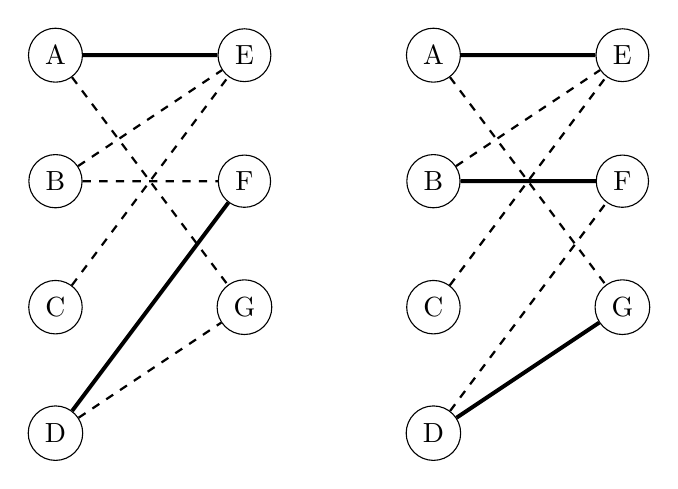
\begin{tikzpicture}[scale=.8,auto=left,every node/.style={circle,draw=black}]
		
		%left nodes
		\node (n1) at (1,10) {A};
		\node (n2) at (1,8) {B};
		\node (n3) at (1,6) {C};
		\node (n4) at (1,4) {D};

		%right nodes
		\node (n5) at (4,10) {E};
		\node (n6) at (4, 8) {F};
		\node (n7) at (4, 6) {G};
		
		%edges
		\draw[line width=0.5mm] (n1) -- (n5);
		\draw[thick,dashed] (n1) -- (n7);
		\draw[thick,dashed] (n2) -- (n5);
		\draw[thick,dashed] (n2) -- (n6);
		\draw[thick,dashed] (n3) -- (n5);
		\draw[line width=0.5mm] (n4) -- (n6);
		\draw[thick,dashed] (n4) -- (n7);

		%left nodes
		\node (m1) at (7,10) {A};
		\node (m2) at (7,8) {B};
		\node (m3) at (7,6) {C};
		\node (m4) at (7,4) {D};

		%right nodes
		\node (m5) at (10,10) {E};
		\node (m6) at (10, 8) {F};
		\node (m7) at (10, 6) {G};
		
		%edges
		\draw[line width=0.5mm] (m1) -- (m5);
		\draw[thick,dashed] (m1) -- (m7);
		\draw[thick,dashed] (m2) -- (m5);
		\draw[line width=0.5mm] (m2) -- (m6);
		\draw[thick,dashed] (m3) -- (m5);
		\draw[thick,dashed] (m4) -- (m6);
		\draw[line width = 0.5mm] (m4) -- (m7);

		\end{tikzpicture}
		\caption{Examples of matchings on a bipartite graph, where bold edges denote those in 
		the matching.}
	\end{figure}
	Oftentimes, we want to find the largest matching on a graph. 
	This is classically motivated by economic examples, where we 
	have a set of bidders and a set of goods, and the edges between them denote a bidder $i$'s 
	willingness to pay for good $j$. For a money-hungry auctioneer, the goal here would be to 
	find the ``largest'' matching on the graph, i.e. the one that maximizes profit of the auction. 
	We will discuss this interpretation in more depth later on in the thesis, but it naturally 
	leads to the following definition.
	\begin{definition}
		A \emph{maximal matching} on $G$ is a matching $M$ such that if any other edge 
		not in $M$ is added to $M$, it is no longer a valid matching. Alternatively put, 
		$M$ is maximal if there is no matching $M\'$ such that $M\subset M\'$.
	\end{definition}
	Both matchings in Figure 1.2 are maximal matchings; in each case, there are no edges that 
	we can add to $M$ and have that $M$ is still a valid matching. However, notice that these 
	matchings have different sizes, even though both are maximal on $G$. This leads to the following 
	definition.
	\begin{definition}
		A matching $M$ on a graph $G$ is said to be a \emph{maximum matching} if for all other 
		matchings $M\'$ on $G$, $|M\'| \leq |M|$.
	\end{definition}
	In our example, the matching on the right given by 
	$M = \{(\mbox{A},\mbox{E}), (\mbox{B},\mbox{F}), (\mbox{D},\mbox{G})\}$ is a 
	maximum matching, since there are no valid matchings such that $|M| > 3$ on this graph. 
	In general there may be many unique maximum matchings on a graph.

	In this section, we are interested in general methods for finding maximum matchings on 
	bipartite graphs. One of the fundamental approaches is to look at certain subgraphs called 
	alternating paths. Before we define what these are, we will first look at a motivating example.
	Suppose that we have the matching $M$ on the left in Figure 1.2. So 
	$M = \{(\mbox{A},\mbox{E}),(\mbox{D},\mbox{F})\}$. 
	Consider the path $p$ of edges and vertices in our graph, shown in Figure 1.3.
	\begin{figure}[h]
		\centering
		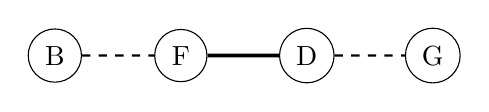
\begin{tikzpicture}[scale=.8,auto=left,every node/.style={circle,draw=black}]

			\node (n1) at (1,10) {B};
			\node (n2) at (3,10) {F};
			\node (n3) at (5,10) {D};
			\node (n4) at (7,10) {G};

			\draw[thick,dashed] (n1) -- (n2); 
			\draw[line width=0.5mm] (n2) -- (n3);
			\draw[thick,dashed] (n3) -- (n4);
		\end{tikzpicture}
		\caption{The path $p$}
	\end{figure}
	Let's perform an 
	operation that we will denote $M\oplus p$, which operates like XOR: add to $M$ each edge in 
	$p$ that isn't in $M$, and remove from $M$ each edge in $p$ that is in $M$. This gives us 
	a new path $p^{'}$, where $(\mbox{B},\mbox{F})$ and $(\mbox{D},\mbox{G})$ 
	are now in $M$, but $(\mbox{D},\mbox{F})$ is not. This new path is shown in Figure 1.4.
	\begin{figure}[h]
		\centering
		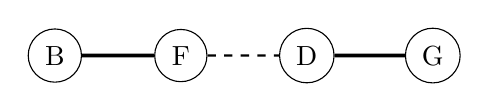
\begin{tikzpicture}[scale=.8,auto=left,every node/.style={circle,draw=black}]

			\node (n1) at (1,10) {B};
			\node (n2) at (3,10) {F};
			\node (n3) at (5,10) {D};
			\node (n4) at (7,10) {G};

			\draw[line width=0.5mm] (n1) -- (n2); 
			\draw[thick,dashed] (n2) -- (n3);
			\draw[line width=0.5mm] (n3) -- (n4);
		\end{tikzpicture}
		\caption{Augmented path $p^{'}$}
	\end{figure}
	First, we must check that the new matching $M\oplus p$ is still a valid matching; 
	we do this by noticing that 
	$\mbox{B}$ and $\mbox{G}$ were originally unmatched, so it's okay for one of their incident 
	edges to be 
	added. Also, notice that the size of our matching has grown by 1! In fact, this new matching 
	is exactly the matching given by the graph on the right in Figure 1.2. 
	
	This is a general technique in 
	finding maximum matchings. We want to look for these paths that start and end at unmatched 
	vertices, and whose edges are alternately matched and unmatched. If we can find one of these 
	paths, we will be able to increase the size of matching by one. We define this formally now.
	\begin{definition}
		Let $G$ be a graph and $M$ be some matching on $G$. An \emph{alternating path} is a 
		sequence of edges that alternate between being matched and unmatched.
	\end{definition}
	\begin{definition}
		An \emph{augmenting path} is an alternating path that starts and ends on unmatched 
		vertices. When we augment $M$ by an augmenting path $p$, we use the notation 
		$M\oplus p$.
	\end{definition}
	This provides a general method for finding a maximum matching on a bipartite graph: 
	look for augmenting paths, and augment the current matching by that augmenting 
	path. The following theorem tells us that this procedure will terminate with a maximum 
	matching.
	\begin{theorem}{(Berge, 1957)}
		A matching $M$ on $G$ is a maximum matching if and only if $G$ contains no augmenting 
		paths with respect to $M$.
	\end{theorem}
	This gives us the following framework for finding maximum matchings in bipartite graphs.
	\begin{figure}
	\begin{center}
		\begin{minipage}{3in}
		\begin{codebox}
			\Procname{$\proc{Maximum matching algorithm} (U,V,E)$}
			\li $M \gets \emptyset $
			\li $\While$ there exists an augmenting path $p$ with respect to $M$:
				\Do
			\li		$M \gets M\oplus p$
				\End
			\li $\Return$ $M$
		\end{codebox}
		\end{minipage}
	\end{center}
		\caption{Algorithm for maximum cardinality matching.}
	\end{figure}
	Students with a background in algorithms will be familiar with this framework. For a detailed 
	treatment of the subleties of this algorithm (known as the Ford-Fulkerson-Method) see Chapter 
	26 of Cormen, Leiserson, Rivest, and Stein \cite{cormen2009introduction}. We will rely on 
	this method of finding maximum cardinality matchings later on in this thesis.
\end{section}

\begin{section}{Linear Programming}
	The development of combinatorial optimization has been deeply intertwined with the discipline 
	of linear programming. 
	A detailed treatment of linear programming can be found in Bertsimas and Tsitsiklis 
	\cite{bertsimas1997introduction} and Vazirani \cite{vazirani2002approximation}.
	For the purposes of this thesis, we will treat linear programming more casually, only focusing 
	a few key results. Moreover, we will not be discussing methods of actually solving linear 
	programs, for which there are at least a couple of well known but complicated algorithms. These 
	are the Ellipsoid algorithm and the Simplex algorithm. An interested reader may find a detailed 
	treatment of these in Papadimitriou and Steiglitz \cite{papadimitriou2013combinatorial}.

	In the general linear-programming problem, our goal is to optimize some linear function that 
	is constrained by a set of linear inequalities. These problems are ubiquitous in applied math 
	and computer science, as they model a system in which something needs to be optimized according 
	to competing resources. We can express a general \emph{maximization} linear program as
	\begin{alignat}{3}
		& \text{maximize } & \sum_{j=1}^{n} c_{j} x_{j}& \\
		& \text{subject to } \quad & \sum_{j=1}^{n} a_{ij} x_{j} & \leq b_{j}, & i & = 1, \dots 
		, m \\
				&& x_{j} & \geq 0, \quad & j & = 1, \dots, n.
	\end{alignat}
	We call the function in (1.1) our \emph{objective function}, and the linear inequalities (1.2) 
	and (1.3) our constraints. Similarly, a \emph{minimization} linear program takes the form
	\begin{alignat}{3}
		& \text{minimize } & \sum_{j=1}^{n} c_{j} x_{j}& \\
		& \text{subject to } \quad & \sum_{j=1}^{n} a_{ij} x_{j} & \geq b_{j}, & i & = 1, \dots 
		, m \\
				&& x_{j} & \geq 0, \quad & j & = 1, \dots, n.
	\end{alignat}
	A possible solution to a linear program is \emph{feasible} if it satisfies all of the linear 
	constraint equations. The following is a simple example from Cormen, Leiserson, Rivest, 
	and Stein \cite{cormen2009introduction} of a linear program:
	\begin{alignat*}{3}
		& \text{maximize } &\quad x_1 + x_2 & \\
		& \text{subject to } &\quad 4x_1 - x_2 &\leq &8 \\
				     && 2x_1 + x_2 &\leq &10 \\
				     && 5x_1 - 2x_2 &\geq &-2 \\
				     && x_1,x_2 & \geq &0.
	\end{alignat*}
	For a simple linear program such as this, one may use basic substituion and elimination methods 
	to get a solution. In this case, it turns out that $x_1 = 2$ and $x_2 = 6$ is an optimal 
	solution. Note that our 
	constraint equations specificy a solution space in $\R^2$. In general, one can imagine 
	$n$-dimensional solution spaces in which more complicated methods are required for 
	finding solutions.

\end{section}
	Many problems which on the face may not appear to be linear optimization problems turn out to be 
	easily rephrased as linear programs. Our goal in the next section will be to describe two 
	problems in terms of their linear programs. The first of these problems will be the is the 
	maximum matching problem. The second will be a problem called the minimum vertex 
	cover problem. Both problems share a very fundamental relationship, which we will discover 
	via their linear programs. We will also revisit a problem that algorithms students are familiar
	with, which is the max-flow min-cut theorem. However, we will approach it from a different 
	perspective using linear programs, which will hopefully demonstrate the cool, deep math 
	that is behind the relationship between flows and cuts.
